\mysection{Principle of Inclusion and Exclusion}

\begin{example}[exp:]{Introduction}
    \eitem{%
        At a school, there are $28$ students in algebra class, 30 students in biology class, and 8 students in both classes. How many students are in either algebra or biology class?
        }{%
        \textbf{Sol:} Let $A$ denote  the  set  of  students  in  algebra  class  and $B$ denote  the  set  of students in biology class. To find the number of students in either class, we first add up the students in each class:
        \[|A|+|B|.\]
        However, this counts the students in both classes twice. Thus we have to subtract them once: $-\left|A\cap B\right|$.This shows
        \begin{alignat*}{1}
            \left|A\cup B\right|&= \left|A\right|+\left|B\right|-\left|A\cap B\right|\\
                                &= 28+30-8=50,
        \end{alignat*}
        so there are 50 students in at least one of the two classes.
        % https://ghoshadi.files.wordpress.com/2019/04/principle-of-inclusion-and-exclusion-holden-lee.pdf
    }

    \eitem{%
        At a school, there are 55 students in either algebra, biology, or chemistry class; 28 students in algebra class; 30 students in biology class; 24 students in chemistry class; 8 students in both algebra and biology; 16 students in both biology and chemistry; 5 students in both algebra and chemistry
        }{%
        \begin{wrapfigure}{r}{0.4\textwidth} %this figure will be at the right
            \centering
            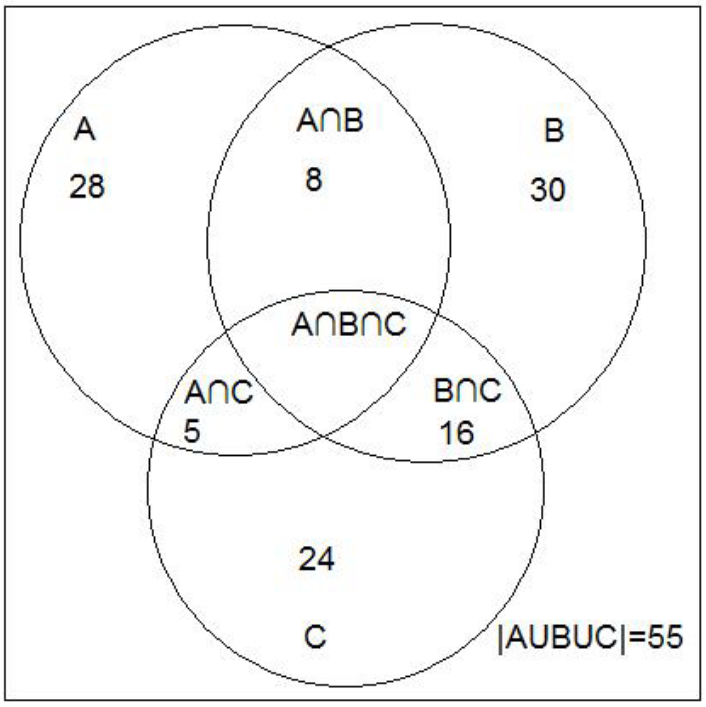
\includegraphics[width=0.9\linewidth]{./pie-p03.png}
        \end{wrapfigure}
        Let $A,B,C$ denote the set of students in algebra, biology, and chemistry class, respectively.  Then $A\cup B\cup C$ is the set of students in one of the three classes, $A\cap B$ is the set of students in both algebra and biology, and so forth. To count the number of students in all three classes, i.e. count $\left|A\cup B\cup C\right|$, we can first add all the number of students in all three classes:
        \[\left|A\right|+\left|B\right|+\left|C\right|.\]
        However, now we’ve counted the students in two classes too many times.  So we subtract out the students who are in each pair of classes:
        \[-\left|A\cap B \right|-\left|B\cap C\right|-\left|A\cap C\right|.\]
    }
    \mynewpage
        For  students  who  are  in  two  classes,  we've  counted  them  twice,  then  subtracted  themonce, so they're counted once.  But for students in all three classes, we counted them 3 times, then subtracted them 3 times.  Thus we need to add them again:
        \[+\left|A\cap B\cap C\right|.\]
        Thus
        \begin{alignat*}{1}
            \left|A\cup B\cup C\right|&= \left|A\right|+\left|B\right|+\left|C\right| -\left|A\cap B \right|-\left|B\cap C\right|-\left|A\cap C\right|+\left|A\cap B\cap C\right|\\
            55 &= 28+30+24-8-16-5+\left|A\cap B\cap C\right|.
        \end{alignat*}
        Thus $\left|A\cap B\cap C\right|=2$, i.e. there are $2$ students in all three classes.
\end{example}

\begin{mysubsection}{Principle of Inclusion-Exclusion}
    \begin{theorem}[thm:]{Principle of Inclusion-Exclusion}
        If $(A_i)_{1\leq i\leq n}$ are finite sets, then:
        \[\left|\bigcup_{i=1}^n A_i\right|=\sum_{i=1}^n\left|A_i\right| -\sum_{i < j}\left|A_i\cap A_j\right| +\sum_{i<j<k}\left|A_i\cap A_j\cap A_k\right|-\cdots\ +(-1)^{n-1} \left|A_1\cap\cdots\cap A_n\right|{}\]
    \end{theorem}

    \begin{proof}
        Consider an element $x\in A_1\cup \cdots \cup A_n$. It is counted once on the left hand side,so we need to show that it is counted once on the right hand side as well.  Suppose $x$ is in the sets $A_{j_{1}},\dots ,A_{j_{m}}$ but not in the rest of the sets. There are ${m\choose k}$ sets $\left\{i_1,\dots ,i_k\right\}$ such that $x\in A_{i_{1}}\cap \cdots \cap A_{i_{k}}$ has to be a subset of $\left\{j_1,\dots ,j_m\right\}$. Thus $x$ is counted ${m\choose k}$ times in the sum $\sum_{1\leq i_1<\cdots <i_k\leq n}^{}\left|A_{i_{1}}\cap \cdots \cap A_{i_{k}}\right|$, and hence is counted
        \[{m\choose 1}-{m\choose 2}+\cdots +(-1)^{m-1}{m\choose m}\]
        on the right hand side. By the Binomial Theorem,
        \[(x+y)^n={n\choose 0}x^ny^0+{n\choose 1}x^{n-1}y^1+\cdots +{n\choose n}x^0y^n,\]
        substitute $x=1,y=-1$, we have
        \begin{alignat*}{1}
            (1-1)^n&= {n\choose 0}-{n\choose 1}+{n\choose 2}-\cdots +(-1)^{n-1}{n\choose n}\\
            1={n\choose 0}&= {n\choose 1}-{n\choose 2}+\cdots +(-1)^{n}{n\choose n}\\
        \end{alignat*}
        Hence $x$ is counted once only in the RHS.
        %https://www.cs.utexas.edu/~tandy/cappello.pdf
    \end{proof}


\mynewpage
\end{mysubsection}

\begin{shortque}[]{}
    \qitem{%
        Find the number of positive integers not exceeding 100 that are not divisible by 5 or 7.
        }{%
        \begin{alignat*}{1}
            \left|A_5\cup A_7\right|&= \left|A_5\right|+\left|A_7\right|-\left|A_5\cap A_7\right|\\
                                    &= \lfloor \frac{100}{5}\rfloor + \lfloor \frac{100}{7}\rfloor-\lfloor\frac{100}{5\cdot 7}\rfloor\\
                                    &= 20+14-2\\
                                    &= 32.
        \end{alignat*}
        The answer is $100-32=68$.
        }{%
        https://www.cs.utexas.edu/~tandy/cappello.pdf
    }

    \qitem{%
        Find the number of positive integers less than or equal to 1000 that aredivisible by 7, 10, or 15.
        }{%
        \begin{alignat*}{1}
            \left|A_7\cup A_{10}\cup A_{15}\right|&= \left|A_7\right|+\left|A_{10}\right|+\left|A_{15}\right|-\left|A_{7}\cap A_{10}\right|-\left|A_{7}\cap A_{15}\right|-\left|A_{10}\cap A_{15}\right|+\left|A_{7}\cap A_{10}\cap A_{15}\right|\\
                                                  &= \lfloor\frac{1000}{7}\rfloor+\lfloor\frac{1000}{10}\rfloor+\lfloor\frac{1000}{15} \rfloor-\lfloor\frac{1000}{70}\rfloor-\lfloor\frac{1000}{105}\rfloor-\lfloor\frac{1000}{30}\rfloor+\lfloor\frac{1000}{210}\rfloor\\
                                                  &= 142+100+66-14-9-33+4\\
                                                  &= 256.
        \end{alignat*}
        }{%
        https://ghoshadi.files.wordpress.com/2019/04/principle-of-inclusion-and-exclusion-holden-lee.pdf
        exp 1.4
    }

    \qitem{%
        A 3-card hand is dealt off of a standard 52-card deck. How many different such hands are there for which all three cards are red or all three cards are face cards?
        }{%
        There are a total of $2\cdot 13$ red cards and $4\cdot 3$ face cards. And $6$ face cards that are red.

        Hence the number equals
        \[\left|A\cup B\right|=\left|A\right|+\left|B\right|-\left|A\cap B\right|={26\choose 3}+{12\choose 3}-{6\choose 3}=2600+220-20=2800.\]
        }{%
        https://math.libretexts.org/Bookshelves/Mathematical_Logic_and_Proof/Book%3A_Book_of_Proof_(Hammack)/03%3A_Counting/3.07%3A_The_Inclusion-Exclusion_Principle
    }
\end{shortque}

\mynewpage

\begin{example}[exp:]{Derangement Introduction}
    \eitem{%
        Suppose there is a deck of $n$ cards numbered from 1 to $n$. Suppose a card numbered $m$ is in the correct position if it is the $m$-th card in the deck. How many ways, $W$, can the cards be shuffled with at least 1 card being in the correct position?
        }{%
    }
\end{example}

\begin{mysubsection}{Probability of Derangement}
    Begin by defining set $A_m$, which is all of the orderings of cards with the $m$th card correct. Then the number of orders, $W$, with at least one card being in the correct position, $m$, by the principle of inclusion–exclusion is
    \[{\displaystyle W=\left|\bigcup _{m=1}^{n}A_{m}\right|=\sum_{i=1}^n\left|A_i\right| -\sum_{i < j}\left|A_i\cap A_j\right| +\sum_{i<j<k}\left|A_i\cap A_j\cap A_k\right|-\cdots\ +(-1)^{n-1} \left|A_1\cap\cdots\cap A_n\right|{}.}\]
    Each value ${\displaystyle A_{m_{1}}\cap \cdots \cap A_{m_{p}}} A_{{m_{1}}}\cap \cdots \cap A_{{m_{p}}}$ represents the set of shuffles having at least $p$ values $m_1,\dots ,m_p$ in the correct position. Note that the number of shuffles with at least $p$ values correct only depends on $p$, not on the particular values of $m$. For example, the number of shuffles having the 1st, 3rd, and 17th cards in the correct position is the same as the number of shuffles having the 2nd, 5th, and 13th cards in the correct positions. It only matters that of the $n$ cards, $3$ were chosen to be in the correct position. Thus there are ${n \choose p}$ equal terms in the $p$th summation.
    \[{\displaystyle W={n \choose 1}|A_{1}|-{n \choose 2}|A_{1}\cap A_{2}|+\cdots +(-1)^{p-1}{n \choose p}|A_{1}\cap \cdots \cap A_{p}|+\cdots }\]
    ${\displaystyle |A_{1}\cap \cdots \cap A_{p}|}$ is the number of orderings having $p$ elements in the correct position, which is equal to the number of ways of ordering the remaining $n - p$ elements, or $(n - p)!$. Thus we finally get:
    \begin{alignat*}{1}
        W&={n \choose 1}(n-1)!-{n \choose 2}(n-2)!+\cdots +(-1)^{p-1}{n \choose p}(n-p)!+\cdots \\&=\sum _{p=1}^{n}(-1)^{p-1}{n \choose p}(n-p)!\\&=\sum _{p=1}^{n}(-1)^{p-1}{\frac {n!}{p!(n-p)!}}(n-p)!\\&=\sum _{p=1}^{n}(-1)^{p-1}{\frac {n!}{p!}}
    \end{alignat*}
    A permutation where no card is in the correct position is called a derangement. Taking $n!$ to be the total number of permutations, the probability $Q$ that a random shuffle produces a derangement is given by
    \[Q=1-{\frac {W}{n!}}=\sum _{{p=0}}^{n}{\frac {(-1)^{p}}{p!}},\]
    a truncation to $n+1$ terms of the Taylor expansion of $e^{-1}$. Thus the probability of guessing an order for a shuffled deck of cards and being incorrect about every card is approximately $e^{-1}$ or $37\%$.
\end{mysubsection}



